\documentclass[12pt]{article}
\usepackage[total={170mm,230mm}]{geometry}

\usepackage{cmap}
\usepackage{hyperref}
\usepackage[utf8]{inputenc}
\usepackage[T2A]{fontenc}
\usepackage[russian]{babel}

\usepackage{graphicx}
\usepackage{xcolor}
\usepackage{amssymb}
\usepackage{amsfonts}
\usepackage{amsmath}
\usepackage{amsthm}
\usepackage{physics}
\usepackage{wrapfig}
\usepackage{cancel}
\usepackage{pdfpages}
\usepackage{hyperref}
\newtheorem{definition}{Опредление}[section]
\newtheorem{theorem}{Теорема}[section]
\newtheorem{axiom}{Аксиома}[section]

\usepackage{pgfplots}
\pgfplotsset{width=7cm,compat=newest}

\usepackage{amsmath}
\DeclareMathOperator\arctanh{arctanh}

\usepackage{amsmath}
\DeclareMathOperator\arccosh{arccosh}

\usepackage{amsmath}
\DeclareMathOperator\const{const}

\title{Курс ядерной физики СПБГУ}

\begin{document}
\maketitle
\newpage
\begin{abstract}
Конспектировал Александр Козлов.
\end{abstract}
\newpage
\tableofcontents
\newpage
\section{Введение}
Данный курс посвящён науке, занимающей изучением мельчайших объектов нашего мира --- атомных ядер. Данная наука охватывает самые разные временные и пространственные масштабы. Ядерные взаимодействия появились после нескольких секунд после рождения Вселенной. С их помощью описываются звёзды, нейтронные звёзды можно рассматривать как большое атомное ядро. 

\par
Ядерная физика~\----~не только ядерная бомба, она охватывает гораздо более широкую область человеческих знаний, это и криминалистика, энергетика, медицина, производство новых материалов и археология. 

\section{Состав атомных ядер. Радиоактивность}
Одно из главных достижений человечества~\----~постижение идеи атомизма, которая заключается в том, что всё из чего\--то состоит. Например, ядра состоят из нуклонов, нуклоны~\----~из протонов и нейтронов, протоны из кварков, кварки взаимодействуют с помощью глюонов и так далее.

\begin{wrapfigure}{R}{0.35\textwidth}
\centering
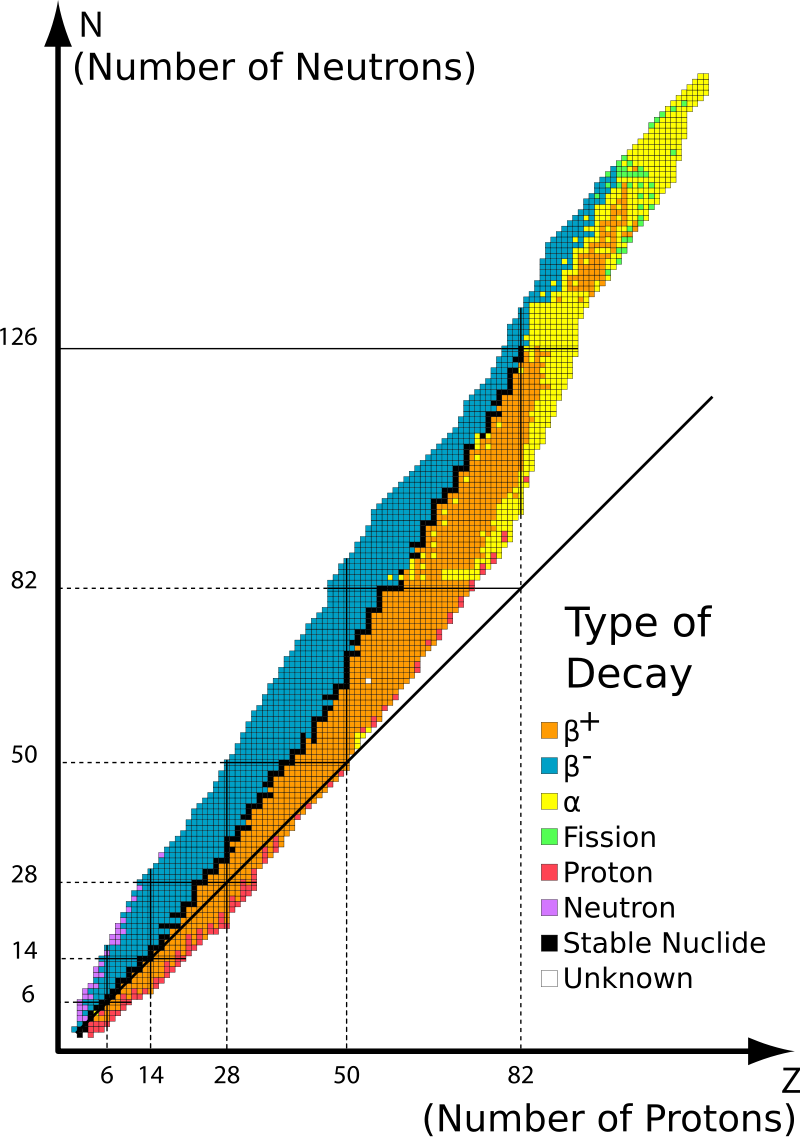
\includegraphics[width=0.3\textwidth]{1.png}
\caption{\label{1}Диаграмма $N \times Z$ радиоактивности}
\end{wrapfigure}

\subsection{Состав атомного ядра}
Атомное ядро есть квантово\--механическая система, поэтому состав атомных ядер определятся той энергией, которую мы рассматриваем, ибо при рассмотрении больших энергий возможен пробой вакуума (рождение электрон-позитронных пар), что приводит к неопределённости состава ядра.

\par
Пускай, под рассмотрением находятся малые энергии. Тогда можно сказать, что атомное ядро состоит из \emph{нуклонов}~\----~протонов и нейтронов. Атомное ядро обозначается элементом, центром которого является ядро. Важными характеристиками ядра являются \emph{массовое число} $A$~\----~число нуклонов в ядре, \emph{зарядовый номер элемента} $Z$~\----~число протонов в ядре и \emph{число нейтронов} $N$. Используется следующий вид обозначения атомного ядра:

\begin{equation}
 {}^{A}_{Z} El_N, \text{где } A = Z + N
\end{equation}

Выделяют следующие типы ядер:
\begin{enumerate}
 \item \emph{Изобары}~\----~ядра с одинаковым числом нуклонов:
 $
 A = \const
 $
 \item \emph{Изотопы}~\----~ядра с одинаковым зарядовым числом:
 $
 Z = \const
 $
 \item \emph{Изотоны}~\----~ядра с одинаковым числом нейтронов:
 $
 N = \const
 $
\end{enumerate}

\subsection{Радиоактивность}
На диаграммах $N \times Z$ все существующие ядра образуют узкую область на диагонали, в середине этой области имеет место быть так называемая \emph{полоса $\beta$\--стабильности}, состоящая из стабильных ядер, по мере удаления от этого островка стабильности время жизни ядер уменьшается и, в конце концов, они вообще перестают существовать. Иными словами, при удалении от полосы $\beta$\--стабильности увеличивается \emph{радиоактивность} ядер.

\subsection{Время жизни ядер}
Основной мерой радиоактивности ядер является время их жизни. \emph{Время жизни ядер} определяется \emph{законом радиоактивного распада}:
\begin{equation}\label{zrr}
 \dd N = -\lambda N \dd t
\end{equation}
Откуда незамедлительно получаем:
\begin{equation}\label{zrr1}
 N\qty(t) = N_0 \exp(-\lambda t)
\end{equation}
В формулах (\ref{zrr}) и (\ref{zrr1}) за $\lambda$ обозначена \emph{вероятность распада}, за $N$~\----~количество оставшихся ядер и за $t$~\----~время, прошедшее с момента, когда количество ядер было равно $N_0$.

\begin{wrapfigure}{R}{0.35\textwidth}
\centering
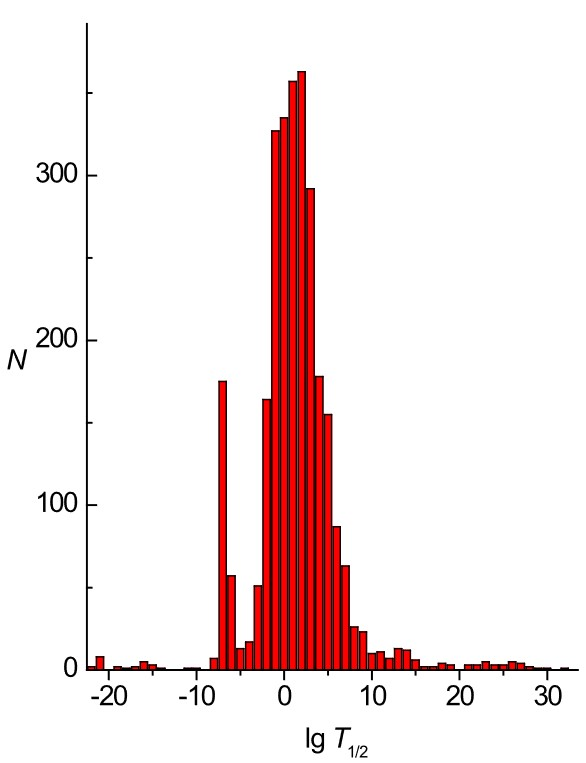
\includegraphics[width=0.3\textwidth]{2.jpg}
\caption{\label{2}Гистограмма периода полураспада ядер}
\end{wrapfigure}

\par
Вероятность распада определяет многие важные на практике характеристики ядра, например, такие, как количество ядер, распавшихся за время $t$:
\begin{equation}
 N_0 - N\qty(t) = N_0\qty(1-\exp(-\lambda t))
\end{equation}
Кроме того, вероятность распада определяет \emph{период полураспада} (период времени, за который успевает распасться половина от исходного количества ядер):
\begin{equation}
 T_{\tfrac{1}{2}} =  \dfrac{\ln{2}}{\lambda}
\end{equation}
На приведённой ниже гистограмме (\ref{2}) показано, что период полураспада ядер может принимать широкий спектр значений от $10^{-23}$ секунд до $10^{30}$ секунд.

\par
Наибольший интерес представляет середина этого набора нуклидов~\----~\emph{стабильные ядра}. На карте нуклидов (\ref{3}) можно видеть несколько сечений по $Z$, то есть несколько химических элементов, содержащие несколько стабильных изотопов (на карте им отвечают чёрные точки). В этом нет ничего удивительного, например, водород представлен двумя стабильными изотопами: протий ${}^1 H$ (просто протон) и дейтерий ${}^2 H$ (протон и нейтрон), кислород~\----~тремя и так далее.

\begin{figure}[ht]
 \centering
 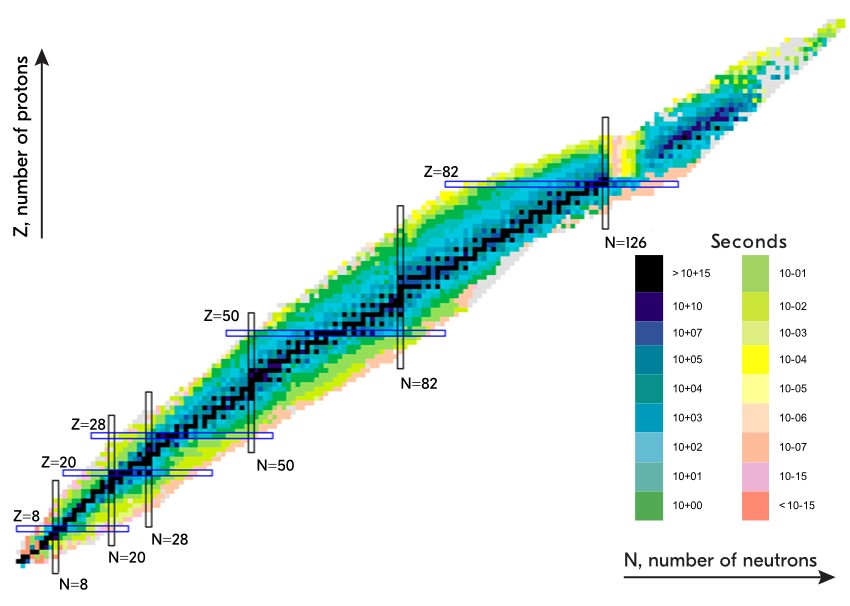
\includegraphics[width = 1\textwidth]{3.jpg}
 \caption{Карта нуклидов.}
 \label{3}
\end{figure}

\section{Массы ядер и энергия связи}
Характеристикой любой физической системы является её масса. Атомное ядро не является исключением. Если масса атома определяется массой ядра, массой электронной оболочки и энергией связи, берущейся из кулоновского взаимодействия, то масса ядра значительно отличается от суммы масс нейтронов и протонов, его составляющих. Так, масса ядра вычисляется следующим образом:
\begin{equation}
\begin{split}
	&M_A \qty(A,Z) = M_N\qty(A,Z) + Z\vdot m_e - B_e \qty(Z),\\
	&B_e\qty(Z) = 14.4381\cross Z^{2.39} + 1.55468\vdot 10^{-6}\cross Z^{5.35}\ [eV].
\end{split}
\end{equation}
Перед тем, как записать формулу вычисления массы ядра, введём новое понятие.
\begin{definition}
	Дефектом масс называется разница между массой ядра и суммой масс нейтронов и протонов, составляющих его.
\end{definition}
Тогда масса ядра вычисляется так:
\begin{equation}
M_N\qty(A,Z) = Z\cross m_p + N \cross m_n - \Delta \qty(A,Z),
\end{equation}
где последнее слагаемое $\Delta \qty(A,Z)$ является дефектом масс. Он бывает достаточно велик, в этом заключается специфика ядра. Так, например, для ядер с $A \sim 200$ дефект масс составляет две массы нуклона, то есть ядро состоящее из $200$ нуклонов имеет массу $198$ нуклонов~\----~такая большая энергия связи.
\par
Через релятивистское соотношение $E = mc^2$ вводится энергия связи. Дадим строгое определение.
\begin{definition}
	Энергия связи, определяемая по формуле
	\begin{equation}
		E_B\qty(A,Z) = \Delta \qty(A,Z),
	\end{equation}
	есть минимальная энергия, необходимая для разделения ядра на составляющие его нуклоны.
\end{definition}
Действительно, чтобы разорвать связь нуклонов, нужно подействовать на них энергией, большей энергии связи либо же равной ей.
\par
Очень удобно ввести понятие удельной энергии связи.
\begin{definition}
	Удельная энергия связи~\----~это энергия связи данного ядра, делённая на число нуклонов, данное ядро составляющих.
\end{definition}
То есть измеренную массу ядра пересчитывают в энергию связи и делят на число нуклонов. На графике \ref{fig:4} представлена зависимость удельной энергии связи от массового числа для всех устойчивых ядер. Стоит обратить внимание на тот факт, что кривая далеко не непрерывная. Существует отдельные ядра, удельная энергия связи которых значительно превосходит удельную энергию связи соседей. К таким ядрам относятся ${}^4 He$, ${}^{12}C$, ${}^{16}O$ и прочие. 
\begin{figure}[ht]
	\centering
	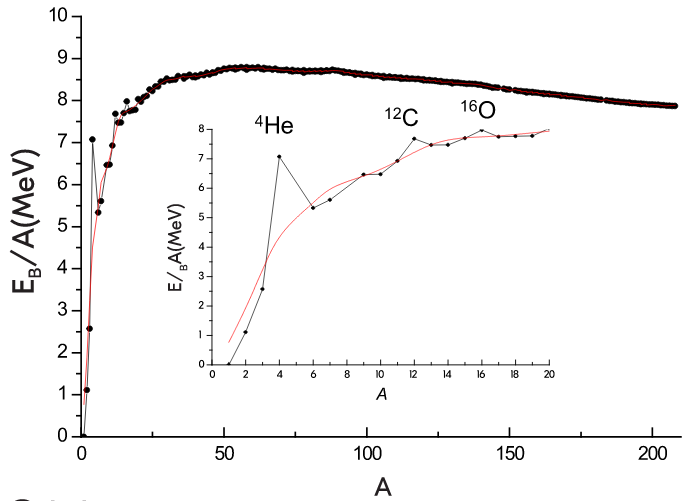
\includegraphics[scale = 0.5]{fig4.png}
	\caption{Удельная энергия связи всех устойчивых ядер.}
	\label{fig:4}
\end{figure}
Кроме того, важно подчеркнуть, что кривая удельных энергий связи имеет характер насыщения. Для тяжёлых ядер с $A$ примерно больше $20$\--$30$ удельная энергия связи выходит на константу. То есть от добавления новых нуклонов энергия связи перестаёт меняться. Данный эффект называется \emph{эффект насыщения ядерных сил}.
\par
У кривой удельной энергии связи есть максимум в районе $A = 56$. Это максимум играет принципиальное значение для приложений ядерной физики, в первую очередь для ядерной энергетики. Если взять ядро с массовым числом $\sim 200$ и разделить его на два элемента, каждый по $\sim 100$, то мы выиграем в энергии. На этом и строиться ядерная энергетика. Также можно заметить, что если слить, например, два ядра водорода в ядро гелия, то будет иметься выигрыш в энергии, правда для того, чтобы обеспечить слияние ядер, нужно разогнать их до крайне высоких энергий. В этом кроется большая проблема и причина слабого развития ядерной энергетики синтеза.
\subsection{Энергии распадов и энергии отдельных частиц}
Порой бывает важным узнать энергии распадов и энергии отделения частиц. Действительно, если есть система из $A$ нуклонов, то какова энергия отделения какого\--либо набора нуклонов. Для этого существуют простые формулы, связанные с массами. Так энергии распадов вычисляются следующим образом:
\begin{equation}
	\begin{split}
	&Q_{\beta -} = M\qty(A,Z) - M\qty(A,Z+1),\\
	&Q_{2\beta -} = M\qty(A,Z) - M\qty(A,Z+2),\\
	&Q_{\alpha} = M\qty(A,Z) - M\qty(A-4,Z-2) - M\qty({}^4 He).
	\end{split}
\end{equation}
Энергии же отделения нуклонов могут быть записаны аналогичным образом:
\begin{equation}
\begin{split}
	&S_{n} = -M\qty(A,Z) + M\qty(A-1,Z) + m_n,\\
	&S_p = -M\qty(A,Z) + M\qty(A-1,Z-1) + m_p,\\
	&S_{2n} = -M\qty(A,Z) + M\qty(A-2,Z) + 2\vdot m_n,\\
	&S_{2p} = -M\qty(A,Z) + M\qty(A-2,Z-2) + 2\vdot m_p.
\end{split}
\end{equation}
Существует сайт \cite{qcalc}, на котором можно с лёгкостью определить энергию распада ядер.
\subsection{Массовые единицы}
Ядерная физика имеет дело с особым классом физических тел, поэтому в ней существует специфичная массовая шкала (либо массовые единицы). За единицу массы в ядерной физике взята $1/12$ массы свободного покоящегося атома ${}^{12}C$, находящегося в основном состоянии:
\begin{equation}
M\qty({}^{12}C) = 12.000\ u.
\end{equation}
В единицах $MeV/c^2$ массовая единица пересчитывается следующим образом:
\begin{equation}
1 u = 0.93144\ MeV/c^2.
\end{equation}
Массы нуклонов пересчитываются в массовых единицах следующим образом:
\begin{equation}
m_n = 939.6\ MeV/c^2 = 1.008665\ u, \quad m_p = 938.3\ MeV/c^2 = 1.007276\ u.
\end{equation}
Стоит помнить, что масса протона и масса атома ${}^1 H$ различны. Приведём примеры масс некоторых атомов, выраженных в атомных единицах массы. Так, например, масса дейтерия будет записываться следующим образом:
\begin{equation}
	M\qty({}^2 H) = 1875.6\ MeV/c^2 = 2.014102\ u,\quad E_B \qty({}^2 H) = 2.224\ MeV.
\end{equation}
Масса альфа\--частицы будет вычислена так:
\begin{equation}
	M\qty({}^4 He) = 3728.0\ MeV/c^2 = 4.002603\ u,\quad E_B \qty({}^4 He) = 28.296\ MeV.
\end{equation}
Для прочих атомов вся информация доступна на сайте \cite{qcalc}.
\subsection{Полуэмпирическая формула масс Бете\--Вайцзеккера}
Для теоретических расчётов массовых характеристик предложена полуэмпирическая формула масс Бете\--Вайцзеккера. Частично она базируется на теоретической капельной модели, частично~\----~на эмпирических данных.
\par
В капельной модели ядро рассматривается как сферическая капля несжимаемой заряженной ядерной жидкости радиуса $R = r_0 A^{{1}/{3}}$. То есть в энергии связи ядра учитываются объемная, поверхностная и кулоновская энергии. Дополнительно учитываются выходящие за рамки чисто капельных представлений энергия симметрии и энергия спаривания. В рамках этой модели можно получить полуэмпирическую формулу Вайцзеккера для энергии связи ядра. Согласно данной модели и эмпирики энергия связи может быть вычислена следующим образом:
\begin{equation}\label{bv}
E_B \qty(A,Z) = \alpha A - \beta A^{\tfrac{2}{3}}- \gamma \dfrac{Z\qty(Z-1)}{A^{\tfrac{1}{3}}} - \delta \dfrac{\qty(A - 2Z)^2}{A} + \zeta A^{-\tfrac{3}{4}}.
\end{equation}
Первое слагаемое в энергии связи ядра, подобного жидкой капле,  пропорционально массовому числу A  и описывает примерное постоянство удельной энергии связи ядер.
\par
Второе слагаемое - поверхностная энергия ядра уменьшает полную энергию связи, так как нуклоны, находящиеся на поверхности имеют меньше связей, чем частицы внутри ядра. Это аналог поверхностного натяжения.
\par
Третье слагаемое в энергии связи обусловлено кулоновским взаимодействием протонов. В капельной модели предполагается, что электрический заряд протонов равномерно распределен внутри сферы радиуса $R = r_0 A^{{1}/{3}}$.
\par
Четвертое слагаемое - энергия симметрии ядра отражает тенденцию к стабильности ядер с $N = Z$.
\par
Пятое слагаемое - энергия спаривания учитывает повышенную стабильность основных состояний ядер с четным числом протонов и/или нейтронов. 
\par 
Входящие в формулу коэффициенты оцениваются из экспериментальных данных по энергиям связи ядер, что дает:
\begin{equation*}
\begin{split}
&\alpha = 15.6\ MeV,\\
&\beta = 17.2\ MeV,\\
&\gamma = 0.72\ MeV,\\
&\delta = 23.6\ MeV,
\end{split}
\end{equation*}
\begin{equation*}
\zeta = 
\begin{cases}
+34\ MeV\ &\text{ч\--ч},\\
0\ MeV\ &\text{н},\\
-34\ MeV\ &\text{н\--н}.
\end{cases}
\end{equation*}
Здесь "ч\--ч"{} обозначает чётно\--чётное ядро (ядро с четным количеством нейтронов и четным количеством протонов), "н"{}~\----~нечётное ядро (ядро с нечётным массовым числом) и "н\--н"{}~\----~нечётно\--нечётное ядро (ядро с нечетным количеством нейтронов и нечетным количеством протонов). 
\begin{figure}[ht]
	\centering
	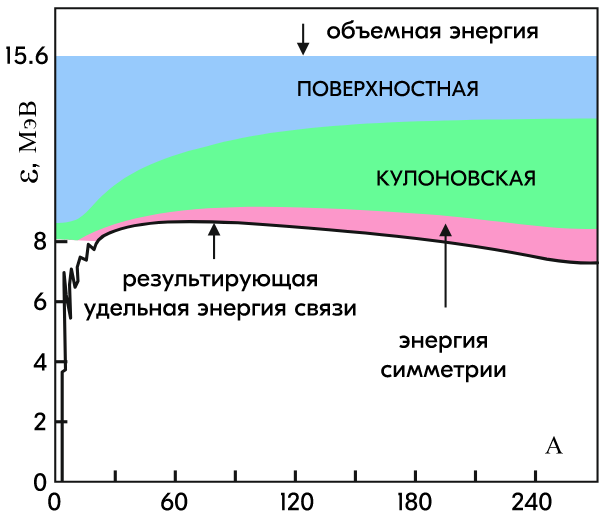
\includegraphics[scale = 0.5]{fig5.png}
	\caption{Иллюстрация к роли слагаемых в формуле (\ref{bv}).}
	\label{fig:5}
\end{figure}
\subsection{Магические числа}
Если мы исследуем разности энергий связи, рассчитанных по формуле (\ref{bv}), которая является гладкой, и дискретных экспериментальных данных, то мы увидим картину, представленную на рисунке \ref{fig:6}.
\begin{figure}[ht]
	\centering
	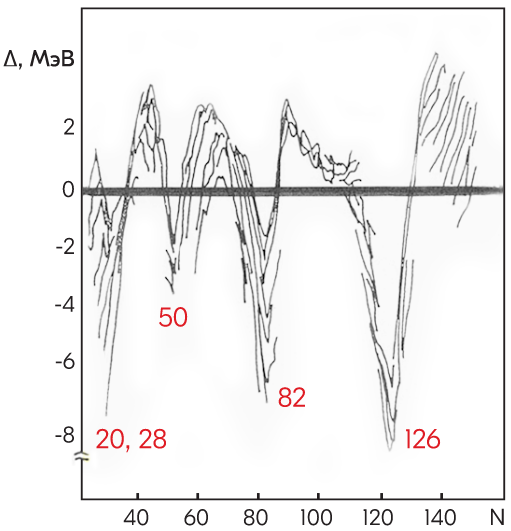
\includegraphics[scale = 0.5]{fig6.png}
	\caption{Разность между экспериментальными энергиями связи и расчётными в зависимости от числа нейтронов.}
	\label{fig:6}
\end{figure}
Видны резкие провалы при числах:
$$
2,8,20,28,50,82,126.
$$
Данные числа получили название \emph{магических}. Они пронизывают всю ядерную физику. Например, магические ядра, отвечающие этим числам, крайне устойчивы и наиболее распространены во Вселенной, поэтому привлекают наибольший интерес исследователей.
\subsection{Выводы}
Говоря о массовых характеристиках ядра, мы установили, что массы атомных ядер отличаются от сумм масс нуклонов, составляющих ядра. Явно прослеживается наличие дефекта масс. Он связан с энергией связи. Энергия связи демонстрирует эффект насыщения ядерных сил (начиная с некоторого массового числа энергия связи перестают расти и достигает насыщения). небольшое убывание энергии связей при больших массовых числах объясняет энергетический эффект, связанный с делением ядер, кроме того объясняет похожий эффект при синтезе ядер. Зная массы ядер, мы можем вычислять энергии отделения частиц от ядра, как работу выхода. Сравнивая экспериментальные значения масс с расчётными по формуле (\ref{bv}), мы углядели, что существует некие особые числа нейтронов и протонов, называемые магическими. Они играют важную роль в ядерной физике.
\section{Размер и форма ядер}


\medskip
\begin{thebibliography}{9}
	\bibitem{qcalc}
	National Nuclear Data Center, QCalculator,
	\\\texttt{\url{https://www.nndc.bnl.gov/qcalc/}}
\end{thebibliography}
\end{document}
